% This text is proprietary.
% It's a part of presentation made by myself.
% It may not used commercial.
% The noncommercial use such as private and study is free
% Sep. 2005
% Author: Sascha Frank
% University Freiburg
% www.informatik.uni-freiburg.de/~frank/
\documentclass{beamer}
\usetheme{Madrid}
\usepackage{palatino}
\usepackage{tikz}
\usetikzlibrary{shapes.geometric, arrows}
\mode<presentation>
{
  \setbeamercovered{transparent}
}
%\logo{\includegraphics[width=1.3cm,height=1.3cm]{duke.png}}
\mode<handout>
{
%%% In handout mode give the individual pages a light grey background
\setbeamercolor{background canvas}{bg=black!5}
%%% Put more than one frame on each page to save paper.
\usepackage{pgfpages}
\pgfpagesuselayout{4 on 1}[letterpaper,border shrink=3mm, landscape]
% \pgfpagesuselayout{2 on 1}[letterpaper,border shrink=5mm, portrait]
% \setbeameroption{show notes}
}
% \usepackage[latin1]{inputenc}
\usepackage[english]{babel}
\begin{document}

\title{Pairs Trading Strategies}
\subtitle{the Optimization in Decision-making Processes}
\author[Group 6]{\scriptsize \emph{Hung-Wei Chang\\Jiaxin Li\\Tianpei Zhu\\Xiaohan Cheng\\Yanlin Chen\\Yuanhang Zhao}}
\subject{Presentation Programs}

\institute[Duke University]{\textbf{Duke University}}
\date{\today}

\frame{\titlepage}

\begin{frame}{Ŀ}%Ŀ¼ %No idea what this is
	\tableofcontents
\end{frame}

\section{Introduction}
\frame{\frametitle{Introduction}
\framesubtitle{Summary}
\textbf{A Combination of All Stages' Optimization.\\}
\begin{block}{\small Decision-Making Processes in Pairs Trading}
\begin{enumerate}\scriptsize
	\item Pairs Selection
	\item Hedge Ratio \& Spread Calculation
    \item Optimal Training \& Stop-Loss Boundaries
    \item Performance Measure
    \item ...
	\end{enumerate}
\end{block}
\textbf{Different Stages, Several Methods to Optimize!\\}
\begin{columns}
\column{.2\textwidth}
\begin{block}{\scriptsize \textbf{Stage 1}}
\tiny
1. PCA\\
2. Machine Learning\\
3. Correlation\\
4. Empirical Criteria\\
5. ...

\end{block}
\column{.2\textwidth}
\begin{block}{\scriptsize \textbf{Stage 2}}
\tiny
1. OLS\\
2. Kalman Filter\\
3. ...

\end{block}
\column{.2\textwidth}
\begin{block}{\scriptsize \textbf{Stage 3}}
\tiny
1. Reinforced Learning\\
2. DQN\\
3. ...

\end{block}
\column{.2\textwidth}
\begin{block}{\scriptsize \textbf{Stage 4}}
\tiny
1. Profit\\
2. Drawdown \\
3. Sharpe Ratio\\
4. ...

\end{block}
\end{columns}
}

\section{Stage Optimization}
\subsection{Pairs Selection}
\frame{\frametitle{Stage Optimization}
\framesubtitle{Pairs Selection - PCA}
\begin{itemize}
\item PCA is a statistical procedure that uses an orthogonal transformation to convert a set of observations of possibly correlated variables into a set of linearly uncorrelated variables, the principal components.
\item Each component can be seen as representing a risk factor.
\item The number of features should not be large.
\item Normalize the return series since PCA is sensitive to the relative scaling of the original variables.
$$Y_{i} = \frac{R_{i}-\bar{R}_{i}}{\sigma_{i}}$$
\end{itemize}
%1. Obtain the return series for a security i at time t , $R_{i,t}$ from the security price %series $P_{i}$
%$$R_{i,t} = \frac{P_{i,t}-P_{i,t-1}}{P_{i,t-1}}$$
}
\frame{\frametitle{Stage Optimization}
\framesubtitle{Pairs Selection - Clustering Methodologies}
\textbf{DBSCAN}
\begin{enumerate}\small
\item  Find the points in the $\epsilon$-neighborhood of every point and identify the core points with more than minPts neighbours, where minPts is a parameter to be tuned.\\
\item  Find the connected components of core points on the neighbour graph, ignoring all non-core points. \\
\item  Assign each non-core point to a nearby cluster if the cluster is an $\epsilon$-neighbor, otherwise assign it to noise.
\end{enumerate}
\begin{figure}[htbp]
    \centering
     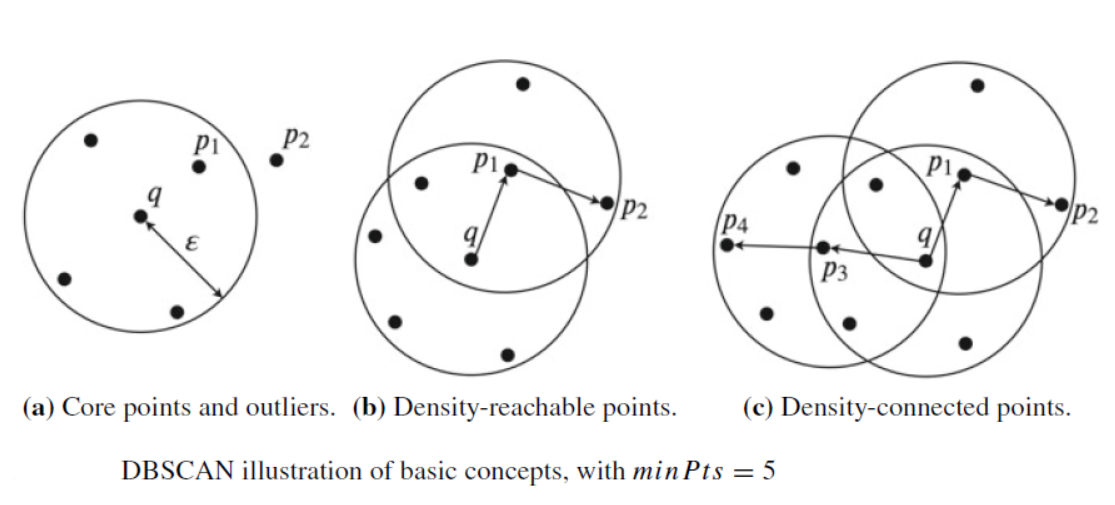
\includegraphics[width=8cm]{3.png}
    \end{figure}
}

\frame{\frametitle{Stage Optimization}
\framesubtitle{Pairs Selection - Clustering Methodologies}
    \begin{figure}[htbp]
    \centering
     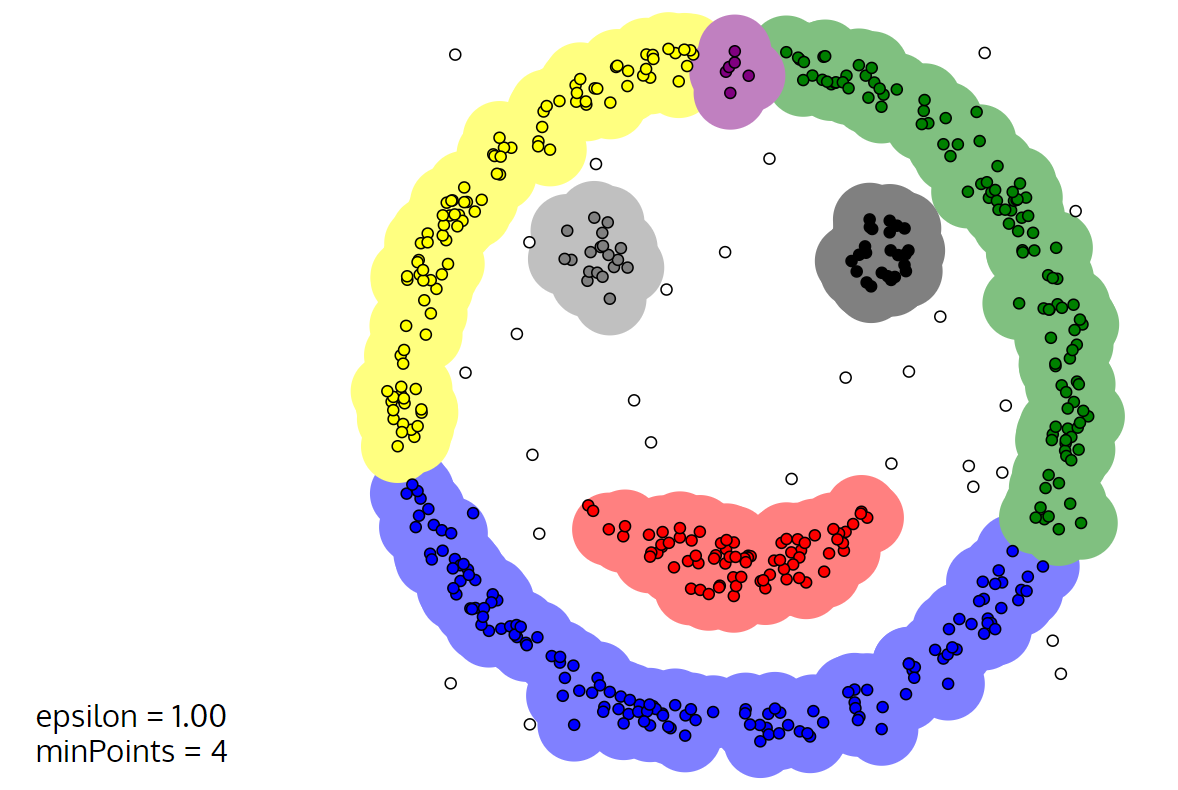
\includegraphics[width=10cm]{9.png}
    \end{figure}
}


\frame{\frametitle{Stage Optimization}
\framesubtitle{Pairs Selection - Clustering Methodologies}
\textbf{OPTICS}
\begin{itemize}\small
\item OPTICS is based on DBSCAN.
\item Appropriate under the assumption that clusters are not evenly dense.
\item Only required to specify the parameter minPts, which is the minimum number of points to form a cluster
\item OPTICS is capable of detecting the most appropriate parameter $\epsilon$, which specifies how close points should be to each other to be considered neighbors.
\end{itemize}
\begin{figure}[htbp]
    \centering
     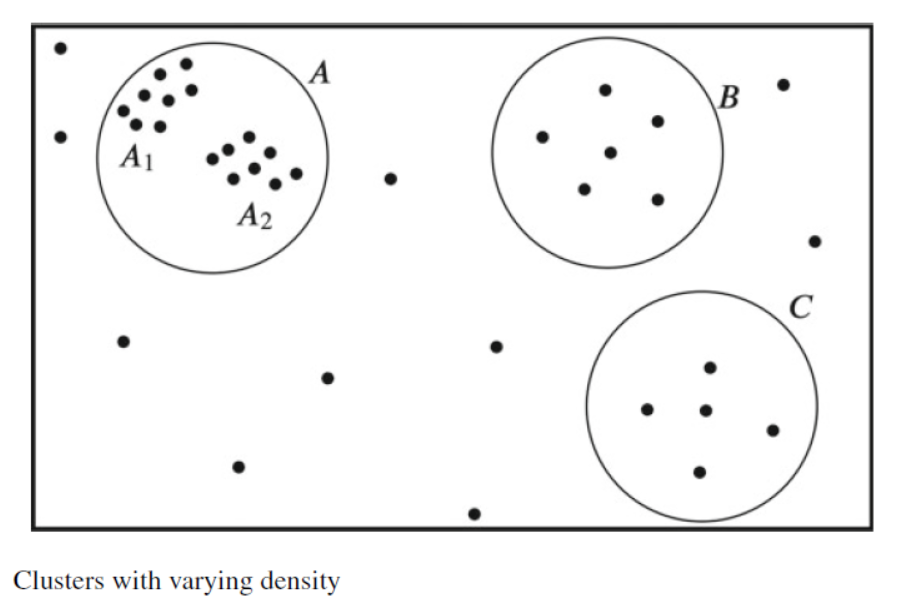
\includegraphics[width=6cm]{4.png}
    \end{figure}
}



\frame{\frametitle{Stage Optimization}
\framesubtitle{Pairs Selection - Other Criteria}
\begin{itemize}
\item Correlation
\item Cointegration
\item Hurst exponent
$$ 
\begin{array}{rcl}
H = 0.5      &     & {random\ walk}\\
H < 0.5      &     & {mean\ reversion}\\
H > 0.5      &     & {persistent\ trend}\\
\end{array}
$$
\item Filter out pairs for which the half-life takes extreme values: less than one day or more than one year.
\end{itemize}
}




\subsection{Hedge Ratio \& Spread Calculation}
\frame{\frametitle{Stage Optimization}
\framesubtitle{One method in Spread Calculation - Kalman Filter}
\begin{block}{A Three-step Process of Prediction, Observation, and Correction}
    \centering corrected\ state = predicted\ state + $k$ (observation\ -\ prediction)
\end{block}
\begin{itemize}
\item (observation - prediction) is called the observation innovation. A fraction of the observation innovation is added as a correction to the predicted state. The value of this fraction $k$ is known as the Kalman gain.
\item $k$ is decided such that the corrected state has the least amount of error variance associated with it.
\item $k$ is indeed optimal in the case where the mathematical models of state and observation are both linear and the errors are drawn from independent Gaussian distributions.

\end{itemize}

}
\frame{\frametitle{Stage Optimization}
\framesubtitle{One method in Spread Calculation - Kalman Filter}
\begin{enumerate}
\item  Evaluate $\hat{X}_{t|t-1}$ and $\hat{P}_{t|t-1}$ using the state equation.
$$ \hat{X}_{t|t-1} = A\hat{X}_{t-1|t-1} $$
$$ \hat{P}_{t|t-1} = A\hat{P}_{t-1|t-1}A^{T} $$
\item  Find the observation $Y_{t}$ and R by observing the system. Note we have the matrix H defined as follows:
$$ Y_{t} = HX_{t} + v_{t}$$
\item Compute the Kalman gain $K_{t}$.
$$ K_{t} = \hat{P}_{t}H^{T}(H\hat{P}_{t}H^{T}+ R )^{-1}$$
\item Evaluate $\hat{X}_{t|t}$ given by
$$ \hat{X}_{t|t} =\hat{X}_{t|t-1} + K_{t}(Y_{t}-H\hat{X}_{t|t-1})$$
\item Evaluate $\hat{P}_{t|t}$
\end{enumerate}
}


\frame{\frametitle{Stage Optimization}
\framesubtitle{One method in Spread Calculation - Kalman Filter}
    \begin{figure}[htbp]
    \centering
     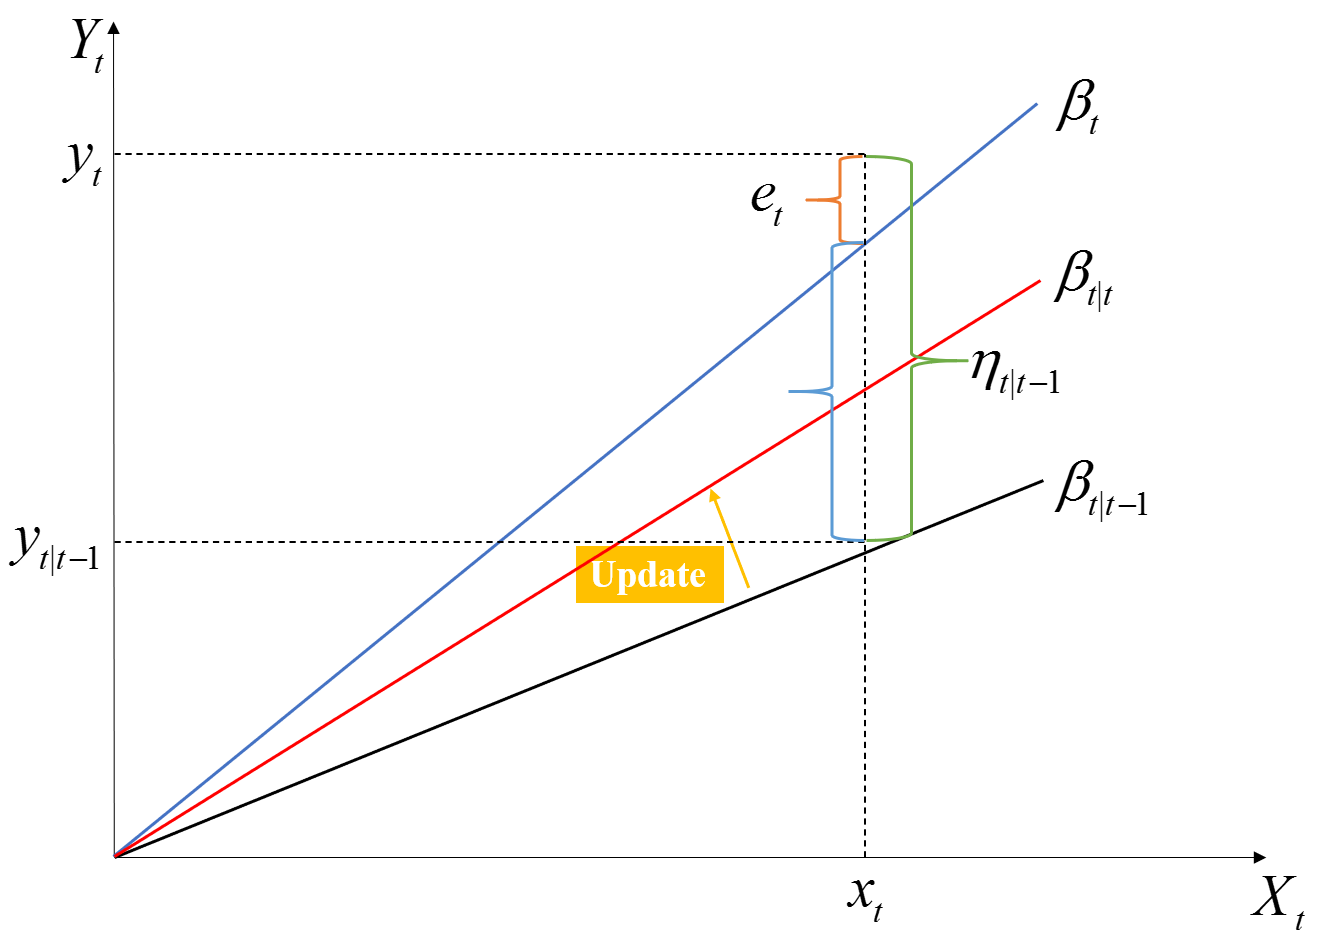
\includegraphics[width=10cm]{5.png}
    \end{figure}
}

\frame{\frametitle{Stage Optimization}
\framesubtitle{One method in Spread Calculation - Kalman Filter}
    \begin{figure}[htbp]
    \centering
     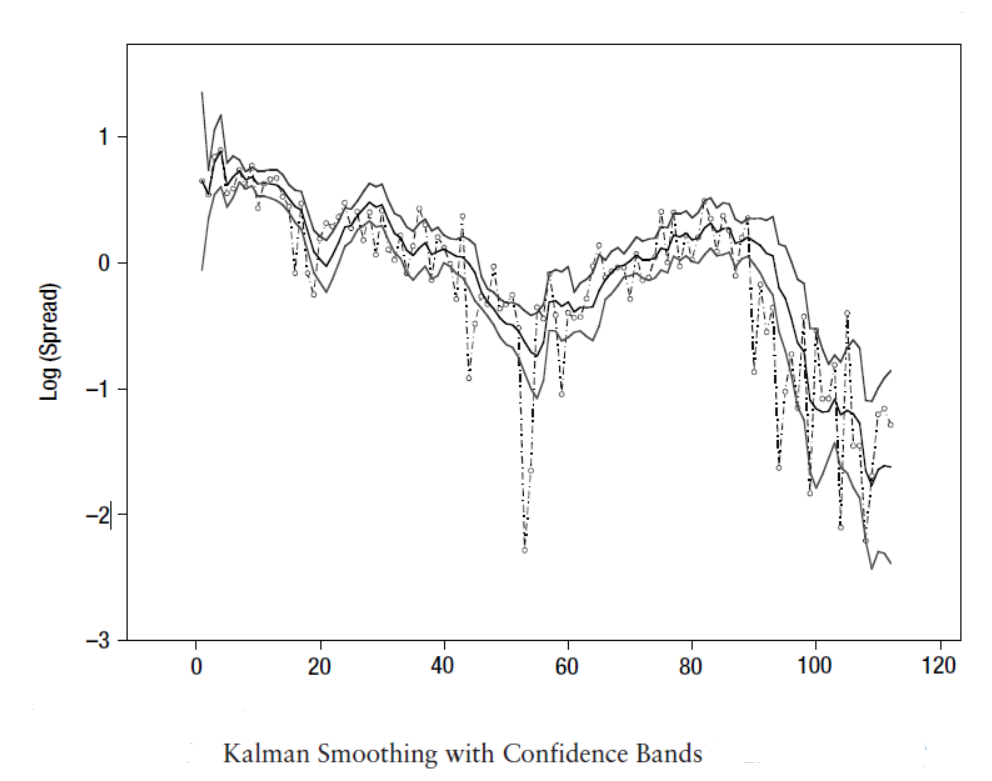
\includegraphics[width=9cm]{7.png}
    \end{figure}
}

\subsection{Optimal Training \& Stop-Loss Boundaries}
\frame{\frametitle{Stage Optimization}
\framesubtitle{Optimal Training \& Stop-Loss Boundaries - DQN Algorithm}
    \begin{columns}
    \column{.5\textwidth}
    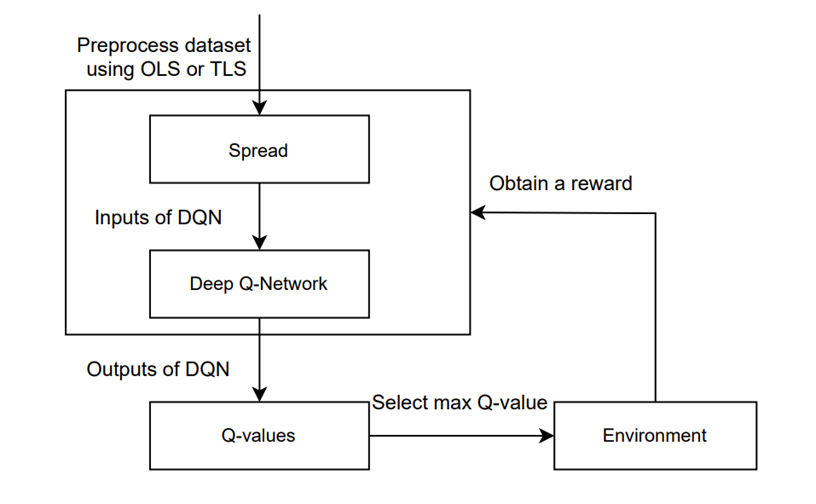
\includegraphics[width=7cm]{2.png}
    \column{.5\textwidth}
    \begin{enumerate}
    \item Get the Spread from OLS or Kalman Filter.
    \item Use DQN algorithm do the iteration for states.
    \item Get the optimal trading actions by reinforced learning
    \end{enumerate}
    \end{columns}
    }
\subsection{Performance Measure}
\frame{\frametitle{Stage Optimization}
\framesubtitle{Performance Measure - From Aspect of Cost management}
    \begin{figure}[htbp]
    \centering
     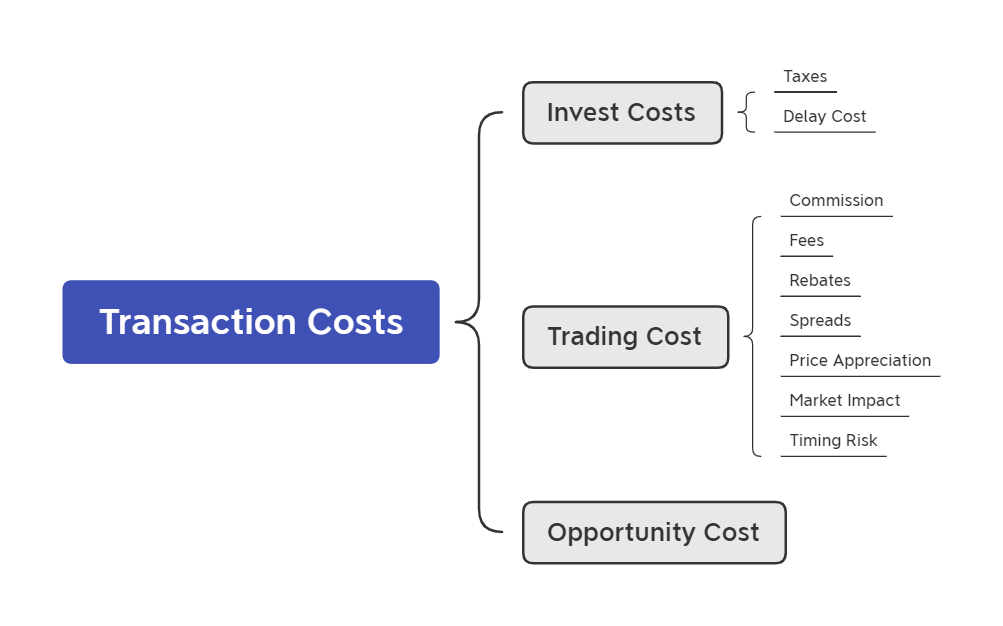
\includegraphics[width=10cm]{6.png}
    \end{figure}
}
\frame{\frametitle{Stage Optimization}
\framesubtitle{Slippage Cost}
\begin{block}{Slippage Cost}
\begin{itemize}
	\item A subset of transaction cost
	\item The cost between listed price and actual pay
	\end{itemize}
\end{block}
\textbf{Eg.}Spread Cost
\begin{itemize}\small
	\item 	Main risk factor: Market Order\\
	   \quad advantage: liquidity\\
	   \quad drawback: bid ask spread may be different at different stock price level
	\item 	Solution: Limit Order\\
	   \quad advantage: full control of the bid-ask spread (we control the execution price)\\
	   \quad drawback: order may never be filled
	\end{itemize}
\textbf{Key point is the balance between execution speed and the control of bid-ask spread!}
}

\section{Performance Measure}
\frame{\frametitle{Performance Measure}
%\framesubtitle{Plan}
\begin{enumerate}
	\item Sharpe Ratio
	\item Calmar Ratio
    \item Jensen's Alpha
    \item Treynor Ratio
    \item Information Ratio
    \item Sortino Ratio
    \item Drawdown \& Maximum Drawdown
    \item Annualized Volatility 
    \item VaR \& Expected Shortfall
    \item Compare our NAV per unit with funds implementing similar strategies.
	\end{enumerate}
}

\section{Future Work}
\frame{\frametitle{Future work}
\framesubtitle{Plan}
\begin{enumerate}
	\item Compare the results from Stage 1 to Stage 3 using different optimal methods.
	\item Find a \textbf{COMBINATION} of all the Optimal Strategies. Child strategies with different assets and weights result in diversification.
    \item We might try different machine learning methods like XGBoost.
	\end{enumerate}
}
\frame{\frametitle{Reference}
\begin{itemize}\scriptsize
\item Simao Moraes Sarmento , Nuno Horta, Enhancing a Pairs Trading strategy with the application of Machine Learning, Expert Systems with Applications, vol 158, 15 November 2020, 113490
\item Gatev, E. G., Goetzmann, W. N., \& Rouwenhorst, K. G. (2006). Pairs Trading: Performance of a Relative-Value Arbitrage Rule. Review of Financial Studies, 19(3), 797C827.
\item Mario, C. B. , De la Orden De la Cruz Carmen, \& Camilo, P. R. . (2018). Pairs trading techniques: an empirical contrast. European Research on Management and Business Economics, 24(3), 160-167.
\item Sarmento, S. M. , \& Horta, N. . (2020). Enhancing a pairs trading strategy with the application of machine learning. Expert Systems with Applications, 158, 113490.
\item Taewook Kim and Ha Young Kim, 2019.
\item Pairs Trading : Quantitative Methods and Analysis Ganapathy Vidyamurthy  (2004)
\item Kissell, R. (2013). The science of algorithmic trading and portfolio management (pp. 87-128). Academic Press.
\item Taylor, Y. (2019). https://seekingalpha.com/article/4256936-minimize-your-slippage
\item https://www.naftaliharris.com/blog/visualizing-dbscan-clustering/
\end{itemize}
}

\end{document}
